\section{Results}\label{sec:results}
Our experiments were carried out on a Red Hat 8 server hosting a Intel Xeon
Gold 6242 CPU. Since \shortname{} is written in Rust, it mostly uses the
built-in functionality of the egg library. The egg e-graph runner was ran in a
time-limited configuration, meaning there was no limit in the size of the
e-graph. Regardless, the median time to saturate a design was 9 seconds.
However, the far majority of results are reached within 20 iterations of
rewriting, and this on average takes only 3 seconds. As for the benchmarks,
\shortname{} was evaluated against circuits from three test suites:
EPFL~\cite{epflbench}, ISCAS'85~\cite{iscasbench}, and
LGSynth'91~\cite{lgsynthbench}. However, we also included an ALU and pipelined
multiplication module to test how our compiler behaves with increasing levels
of bit-parallelism and register pipelining. Finally, we measure how our
remapping optimizations influence CLB usage.

\begin{table}
    \centering
    \caption{Results of \nimproved{} improved benchmarks from ISCAS'85, LGSynth'91, and EPFL. The percent improvements use Vivado as the baseline.}\label{tab:results}
    \csvautobooktabular{data/results.csv}
\end{table}

\begin{figure}
    \begin{subfigure}{0.47\textwidth}
        \centering
        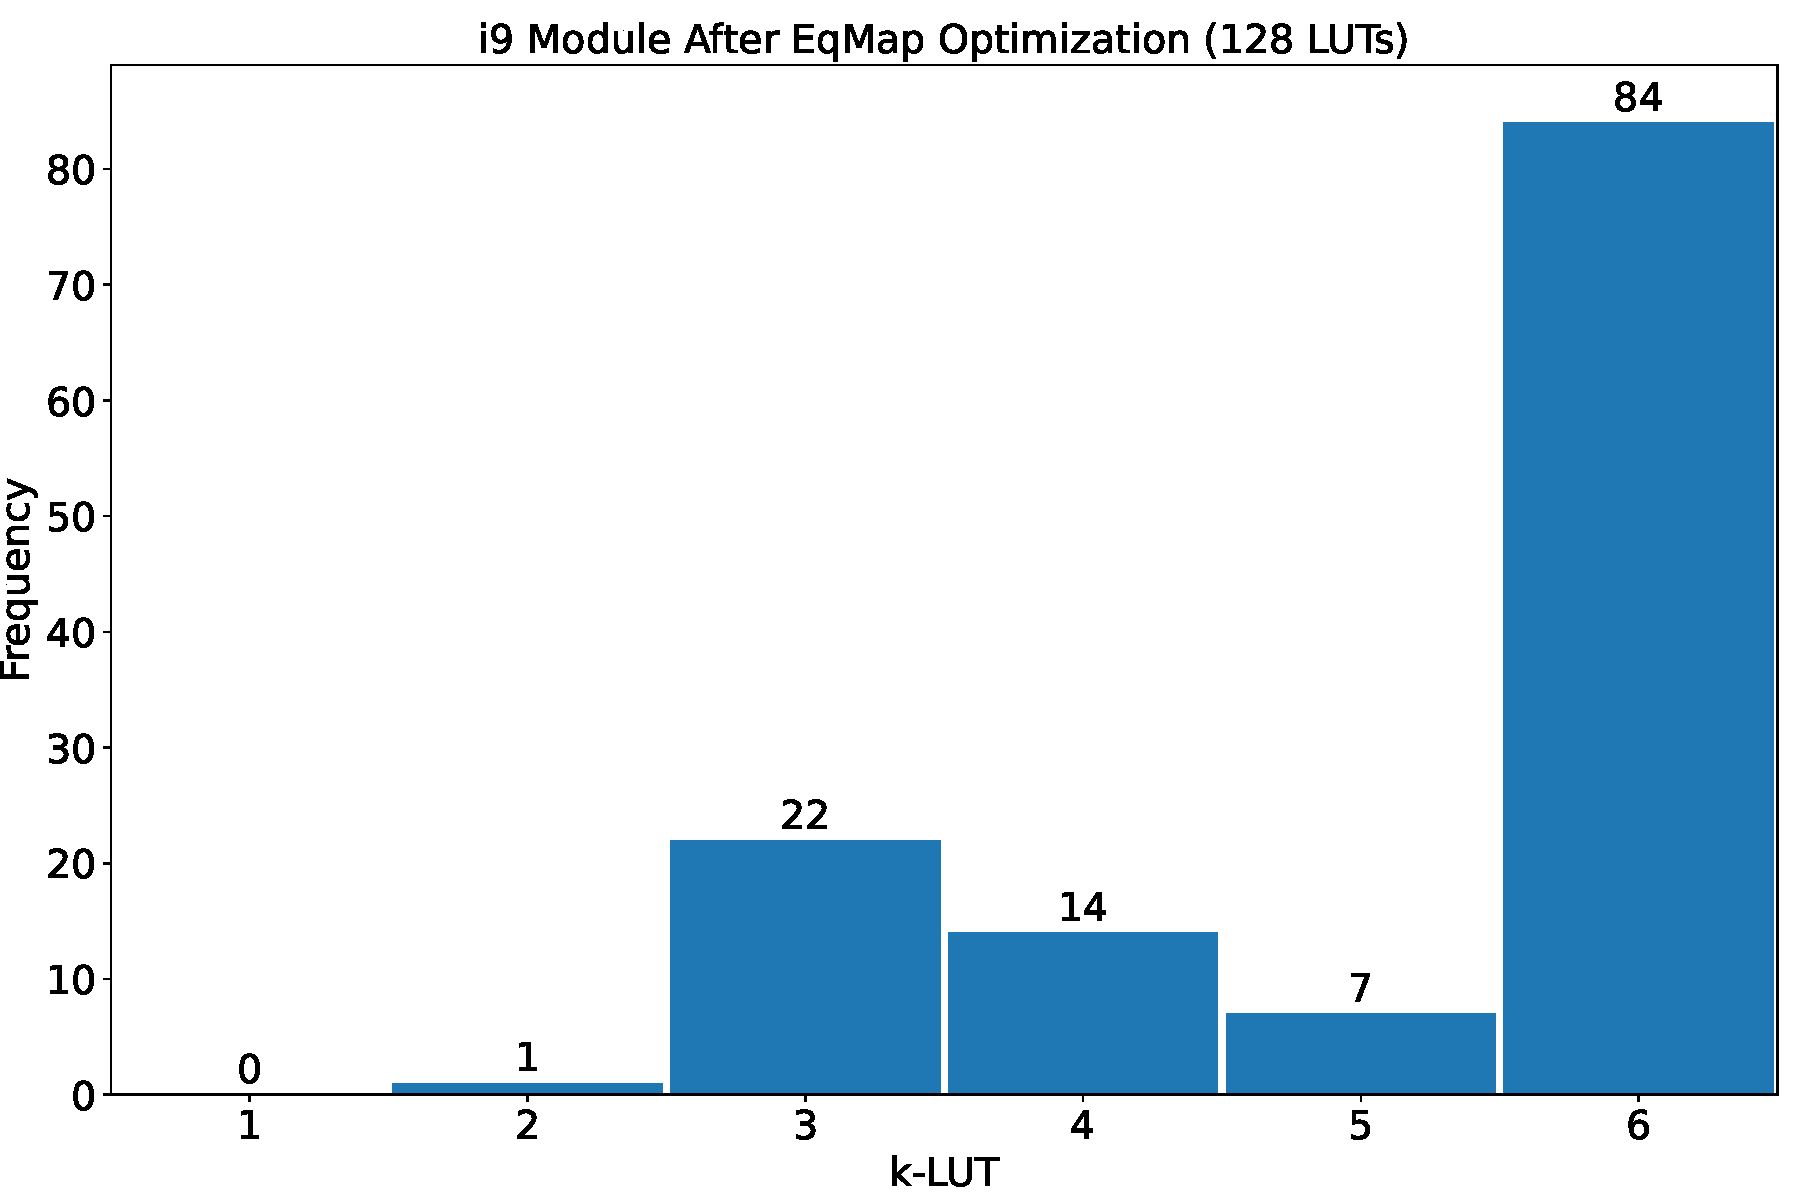
\includegraphics[width=\textwidth]{img/y33.pdf}
        \caption{Distribution of LUTs when using EqMap + Yosys 0.33.}\label{fig:histogram:y33}
    \end{subfigure}
    \hfill\vspace{4mm}
    \begin{subfigure}{0.47\textwidth}
        \centering
        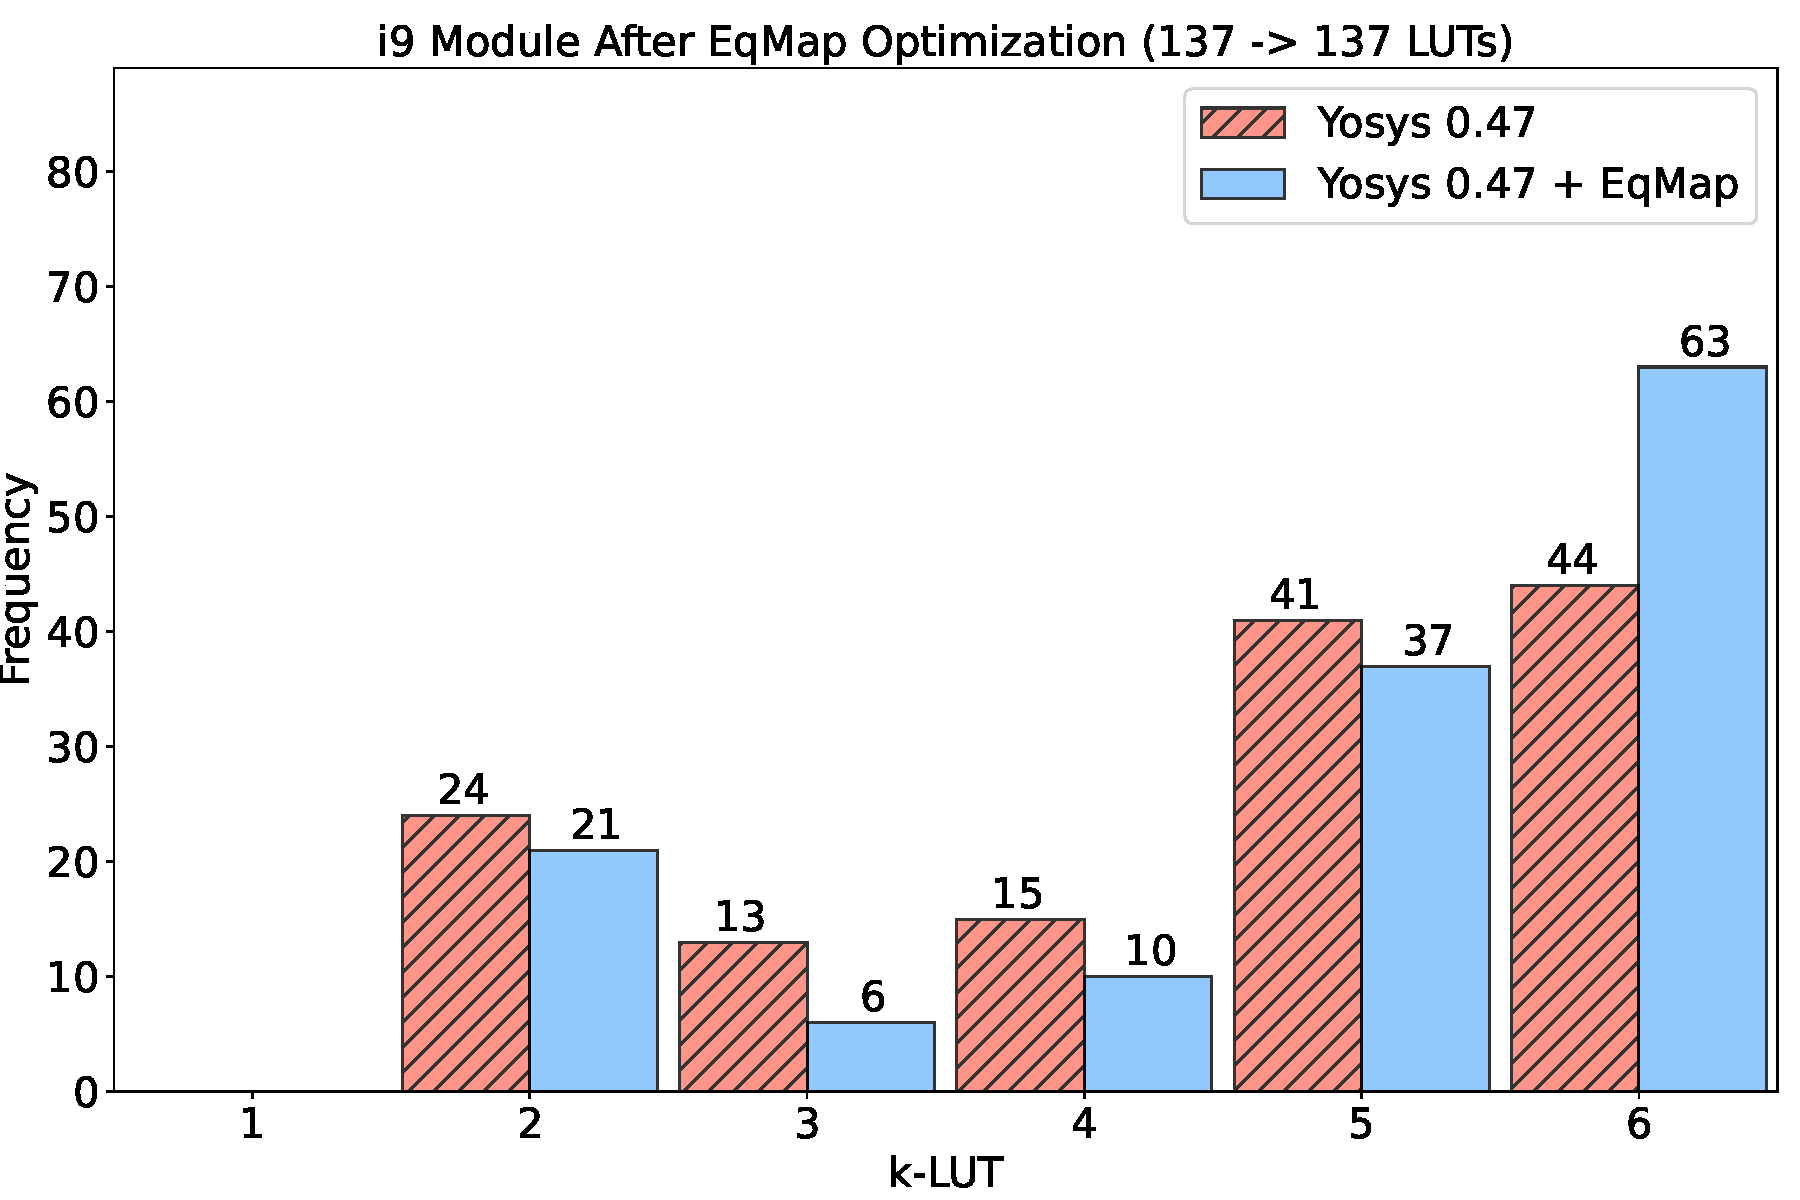
\includegraphics[width=\textwidth]{img/y47.pdf}
        \caption{Distribution of LUTs when using EqMap + Yosys 0.47.}\label{fig:histogram:y47}
    \end{subfigure}
    \caption{Yosys 0.47 maps `i9' with fewer LUTs than Yosys 0.33. However, remapping with EqMap causes the trend to invert.}\label{fig:histogram}
\end{figure}

\subsection{Benchmarking}\label{sec:results:benchmark}

We used a compilation of \nbenchmarks{} combinational benchmarks from three
academic sources to test LUT mapping ability. Among the combinational
benchmarks we tested, \shortname{} was able to reduce the LUT count \fmetric{}
of the time. On average, \shortname{} packed the netlists to \metric{}. The
results in Table~\ref{tab:results} list all the reduced LUT counts, sorted by
approximate design size. AMD/Xilinx Vivado 2024~\cite{vivado} was used as the
baseline synthesis tool. For the \shortname{} flow, Yosys~\cite{yosys} was used
to generate the initial mapped circuit. At a glance, circuits like `int2float,'
`c6288,` `adder,' and `square' have the most to gain from \shortname{}. These
circuits are all arithmetic in nature, and this pattern continues throughout
the rest of the results.

One result that is \textit{not} demonstrated by the table is the apparent
importance of the initial structure inputted to \shortname{}. We have not
eliminated all sources of structural bias, and hence our superoptimization tool
still occasionally gets stuck at a local minimum. Fig.~\ref{fig:histogram}
illustrates the issue by depicting the different distributions of $k$-LUT usage
by different tool flows. In short, an overly packed LUT network will fare worse
in attempts to superoptimize it. Future work will investigate which qualities
make an RTL synthesis engine work well with our tool versus ones that do not.
For example, \shortname{} optimized Yosys 0.33 netlists
(Fig.~\ref{fig:histogram:y33}) better than ones provided by Yosys version 0.47
(Fig.~\ref{fig:histogram:y47}). A future version of \shortname{} should
implement new rewrite procedures than can break out of these local minimums on
their own.

\begin{figure}
    \begin{subfigure}{0.47\textwidth}
        \centering
        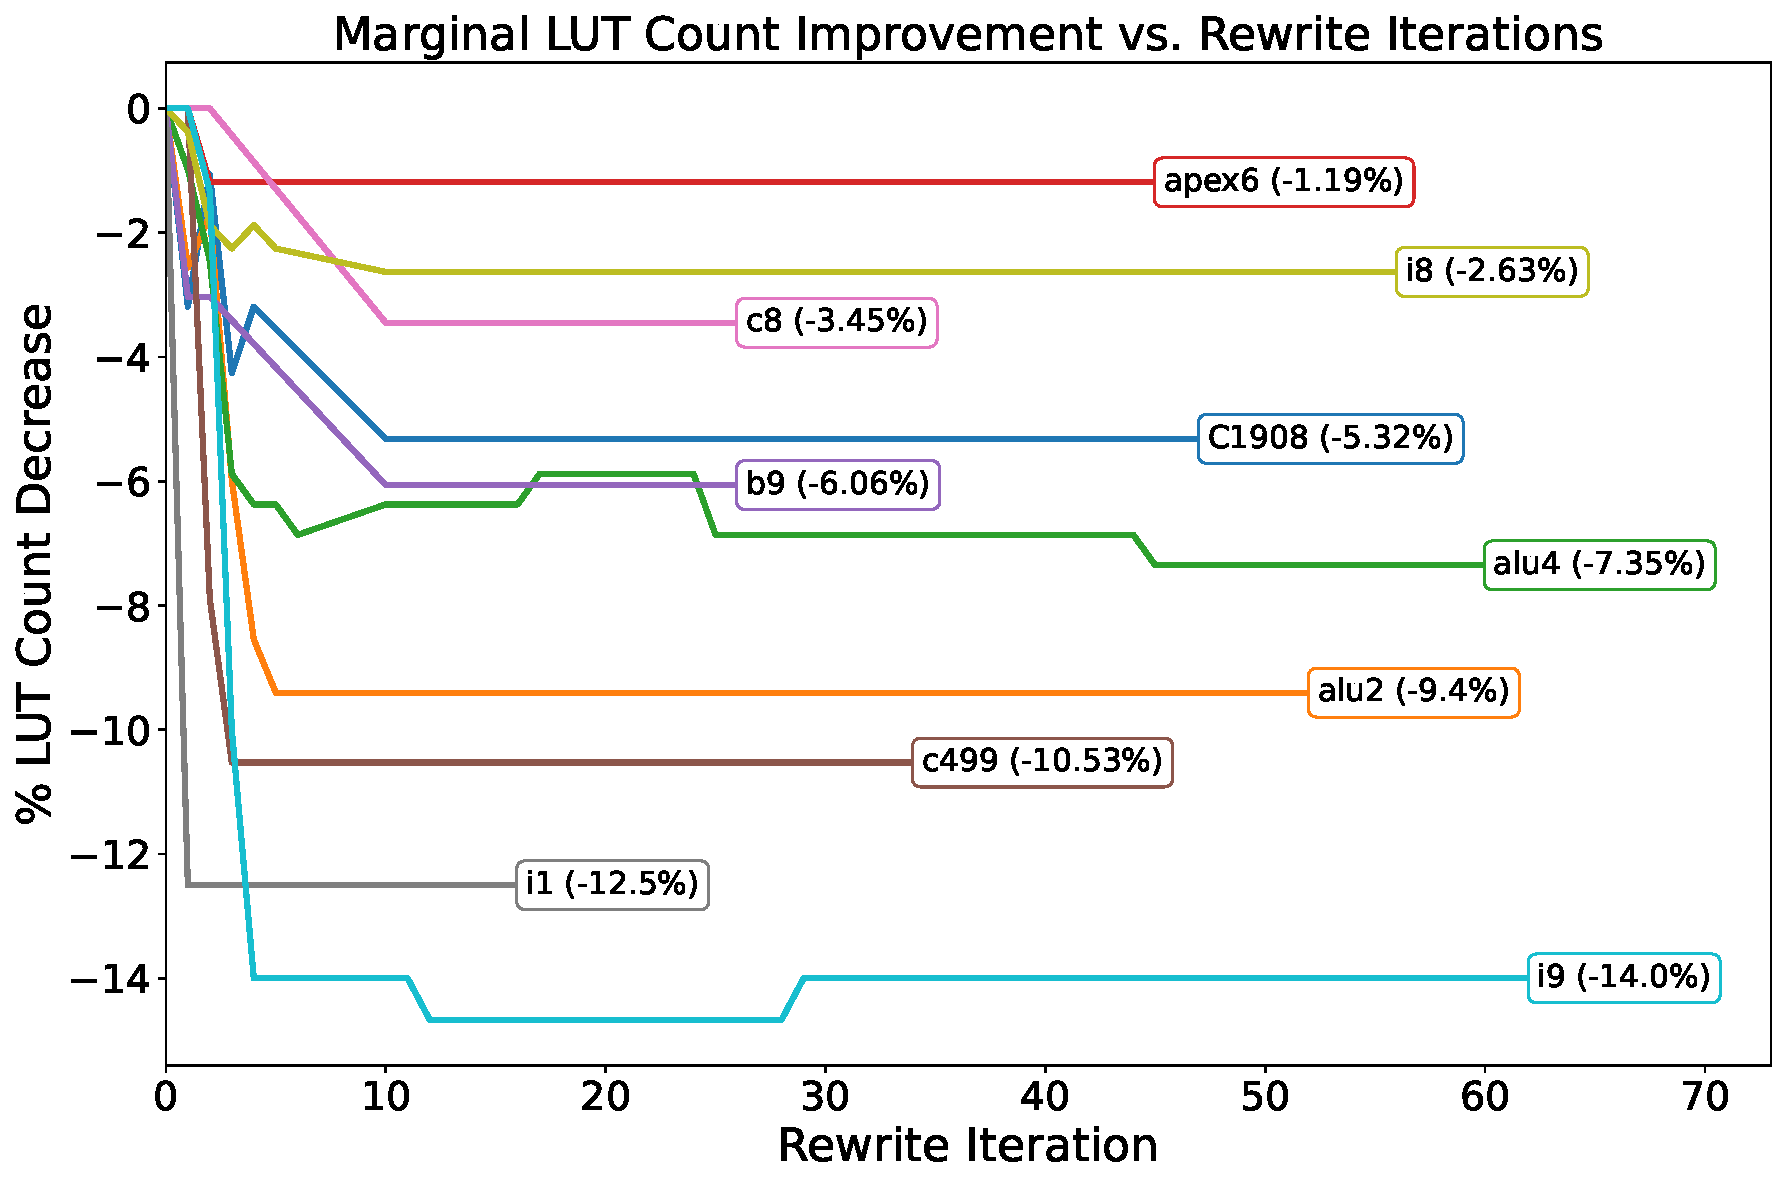
\includegraphics[width=\textwidth]{img/improvement.pdf}
        \caption{Marginal improvement versus iteration count. The labels mark equality saturation.}\label{fig:marginal:improvement}
    \end{subfigure}
    \hfill\vspace{4mm}
    \begin{subfigure}{0.47\textwidth}
        \centering
        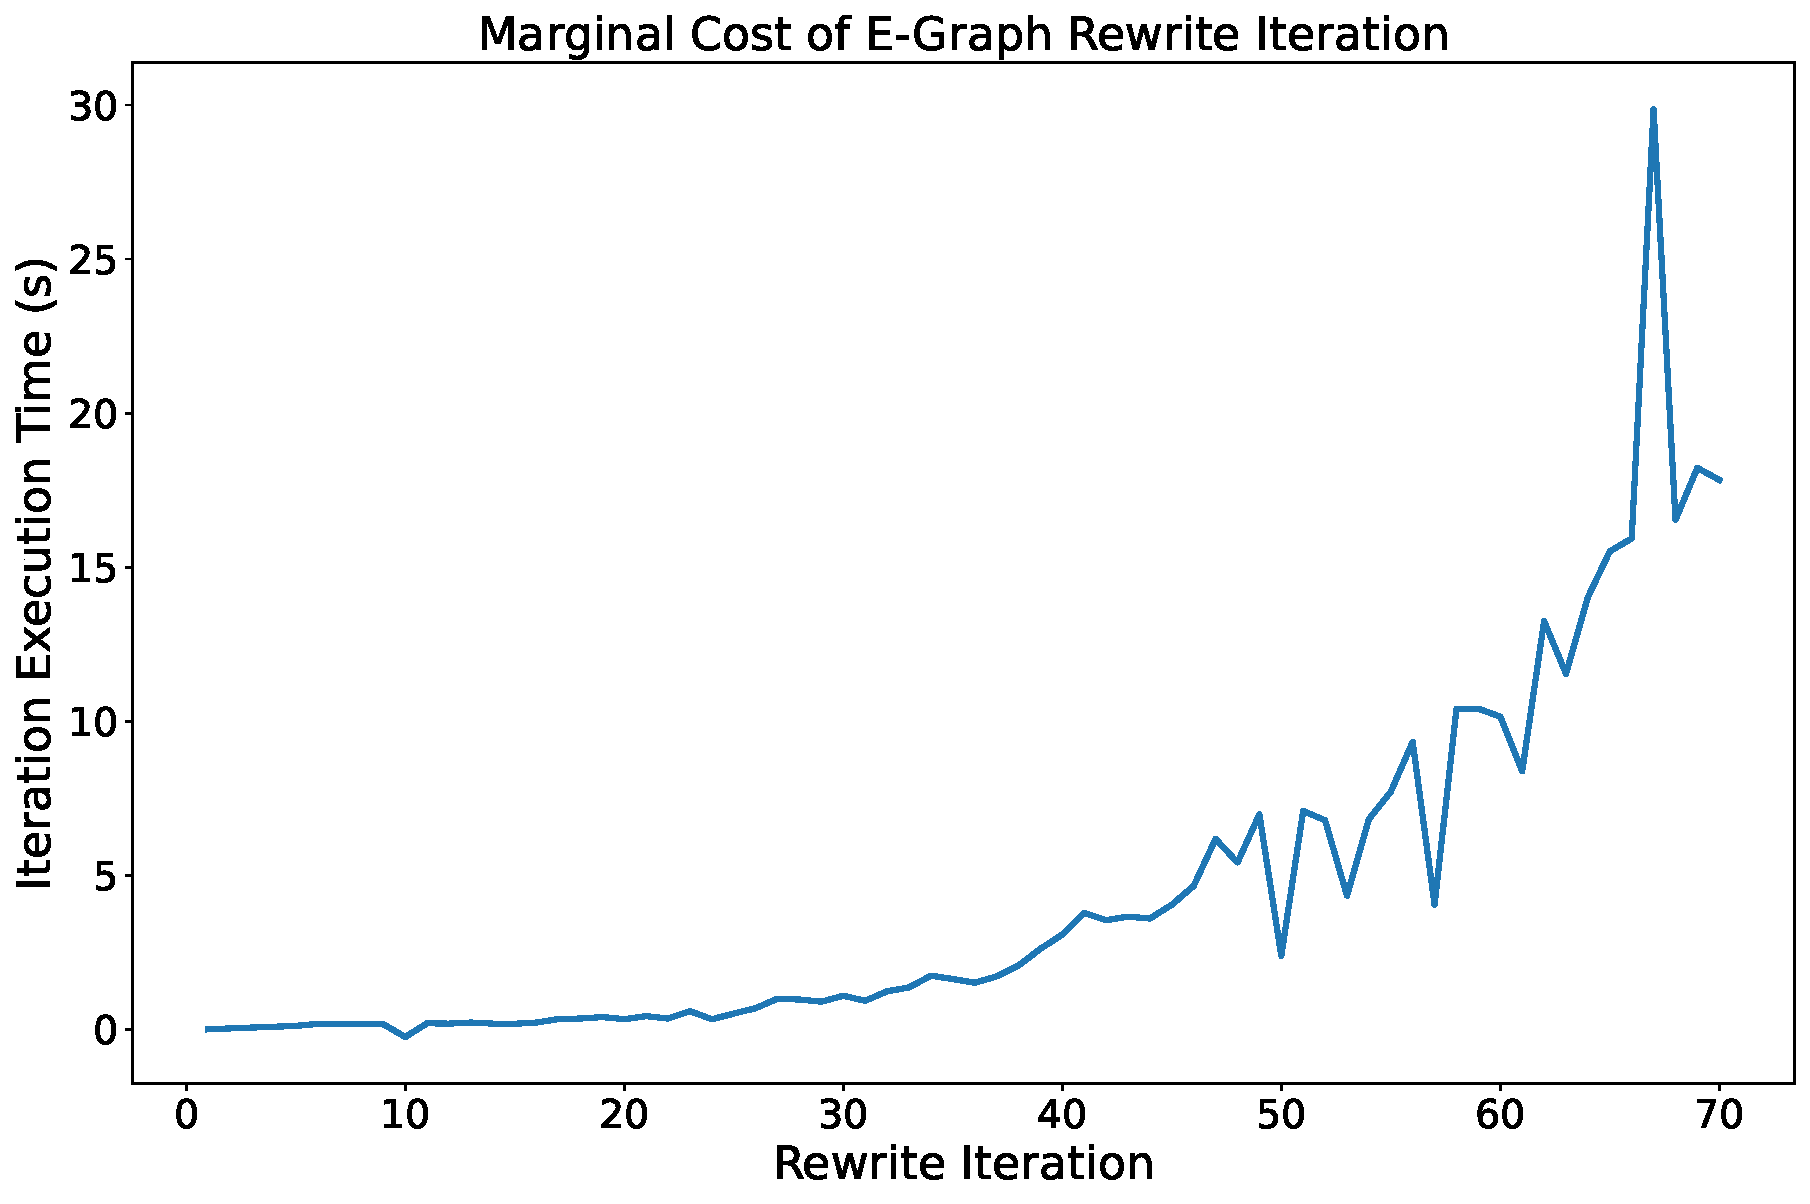
\includegraphics[width=\textwidth]{img/runtime_derivative.pdf}
        \caption{Marginal increase in run time versus iteration count. Later iterations consume more time as the e-graph is larger.}\label{fig:marginal:runtime}
    \end{subfigure}
    \caption{Comparison of marginal gain in QoR against e-graph size and runtime. In most cases, exploring a circuit to equality saturation is not necessary.}\label{fig:marginal}
\end{figure}

\begin{table*}[t]
    \centering
    \caption{Post-implementation results of pipelined multiplication circuit optimized with EqMap. Yosys 0.33 + EqMap is used for synthesis, and Vivado 2024 is used for placement and routing.}\label{tab:multiply}
    \csvautobooktabular{data/mult.csv}
\end{table*}

\subsection{Marginal Improvement and Cost}\label{sec:results:margin}

Given that \shortname{} is fundamentally a superoptimization tool, we want to
provide evidence that significant gains can be found within reasonable time
bounds. To that end, we empirically studied the marginal gains in QoR as
increasingly longer rewrite sequences are added to the e-graph. Within the
e-graph infrastructure, this phasing of applying rewrites and rebuilding the
union-find data structure is referred to as an \textit{iteration}. As shown in
Fig.~\ref{fig:marginal:improvement}, nearly all the performance gains are
discovered within the first 10 iterations---well before equality
saturation---suggesting that most of the optimizations are relatively local.
Some notable exceptions occur, such as `alu4' being reduced in size after the
40th iteration. Lastly, the growing runtime of e-graph exploration with each
iteration should be addressed. The marginal cost of executing an iteration of
rewrites becomes prohibitive as the e-graph becomes larger.
Fig.~\ref{fig:marginal:runtime} illustrates that after approximately the 30th
iteration, the marginal cost in compile time rapidly increases.

\subsection{Case Study: Pipelined Designs}\label{sec:results:retiming}

Hardware designs with feed forward pipelines provide interesting opportunities
to find a higher-level of area optimization. When closing timing on FPGA
designs, the critical path is often dominated by routing, more so than ASIC
design. Hence, reducing the cell count and circuit depth along the max delay
path is a valid optimization strategy for FPGA design. As a caveat, it is
important to note that other work has also observed the opposite
trend~\cite{academicfpga}: decreasing depth too much can strain the router. In
any case, \shortname{} can be utilized to reduce total CLB usage in pipelined
designs. To test this hypothesis, our compiler was used to optimize a 32-bit
integer multiplier with a varying number of pipeline stages. The data in
Table~\ref{tab:multiply} clearly shows that as the number of pipeline stages
increases, some inefficiency in technology mapping is accumulated. \shortname{}
is able to repack the LUTs into roughly the same amount of logic as the single
stage design---without increasing the number of flip-flops. While our current
technique only supports acyclic designs, we wanted to add an additional case
study on pipelined logic to prove the potential of extending our approach
beyond combinational logic.

While the drop in CLB usage is desirable, we anticipate that more exact
extraction techniques would find even greater area reductions. Unlike other
logic rewrites, register retiming changes the topology of the stateful
elements---i.e. the flip-flops. Consequently, greedy extraction cannot take
into account the fan-out these flip-flops. While these results \textit{do}
demonstrate that optimizing for CLB count over raw cell count is a feasible
strategy, a different extraction method will be needed.

\subsection{Case Study: Bit-Parallel Designs}\label{sec:results:scalability}

While the academic benchmarks enable direct comparisons to the rest of the
literature, the circuits are relatively small. On average, the designs map to
670 LUTs. Among the \nimproved{} improved benchmarks in
Table~\ref{tab:results}, only six exceed 1000 LUTs. Although this e-graph
driven technology provides promising results for smaller benchmarks, FPGA
technology mapping is especially difficult---and important---for larger designs
with tens of thousands of LUTs. Through our case study on bit-parallel designs,
we demonstrate that \shortname{} performs just as well on large designs,
achieving area reductions without incurring excessive build times.

To test how \shortname{} scales with increasing numbers of LUTs, we created a
synthetic ALU benchmark and varied the input and output bit widths from 8 bits
to 4096 bits. Table~\ref{tab:alu} lists the LUT counts from the initial
synthesis by Vivado 2024, followed by the packed LUT counts. Even though the
1024-bit, 2048-bit, and 4096-bit ALU designs had up to 15,000 LUTs,
\shortname{} was able to achieve up to almost 15\% improvement over Vivado
within 5 minutes of extra build time. While longer runs lead to slightly better
improvements, these results demonstrate how \shortname{} can achieve area
reductions within a short period of time, even when input designs are scaled to
beyond 10,000 LUTs. In this specific case, \shortname{} can be used to audit
synthesis tools and perhaps even reverse-engineer adverse behavior. Hence,
\shortname{} proves to be a practical tool to run after a baseline synthesis by
Vivado or Yosys to quickly achieve better LUT packing with minimal time cost.

\begin{table}
    \centering
    \caption{EqMap synthesis results of $n$-bit ALU}\label{tab:alu}
    \csvautobooktabular{data/alu.csv}
\end{table}